\begin{abstract}
    Miscalibration of a model is defined as the mismatch between predicting probability estimates and the true correctness likelihood. In this work, we aim to replicate the results reported by \cite{onmixup} on their analysis of the effect of Mixup \cite{mixup_2018} on a network's calibration. Mixup is an effective yet simple approach of data augmentation, which generates a convex combination of a pair of training images and their corresponding labels as the input and target for training a network. We replicate the results reported by the authors for CIFAR-100 \cite{cifar100}, Fashion-MNIST \cite{fmnist}, STL-10 \cite{stl10}, out-of-distribution and random noise data. Our implementation code can be found at \url{https://github.com/MacroMayhem/OnMixup}.
  \end{abstract}

\section{Introduction}
  
\subsection{Calibration}
Modern neural networks are miscalibrated, i.e.\ their predicted confidence value is not reflective of its confidence in prediction. If a model is overconfident, it becomes prone to making wrong predictions with high confidence, thereby depleting the trust on its predictions. It becomes really important in high risk applications (such as in medical diagnosis, automated navigation, etc.) for the neural network's prediction to be correct as well as trustworthy. If the network generates reliable predictions, it would enable the use of some form of fall back mechanism, such as a human-in-the-loop for life critical scenarios. Finding a solution to this problem of miscalibration hence becomes important due to the widespread applicability of deep neural networks %(DNNs) 
across multitude of domains.

Figure \ref{fig:hypothesis} displays this phenomenon where the average accuracy and average confidence is computed per interval bin (see section \ref{sec:metrics} for details). The top row (a--e) corresponds to a training scenario where no Mixup is used. As the training progresses the network tends to become overconfident in its predictions. %However
On the other hand, by training with Mixup, the network is much better calibrated, as can be seen in the bottom row (f--j). Note that the network used to generate the results in fig \ref{fig:hypothesis} is different from the original paper, which uses a VGG-16 architecture. However, the underlying message i.e.\ over confident predictions are avoided when using Mixup is conveyed nonetheless.  
\begin{figure}[htb]
     \centering
     \begin{subfigure}[b]{0.19\textwidth}
         \centering
         \noindent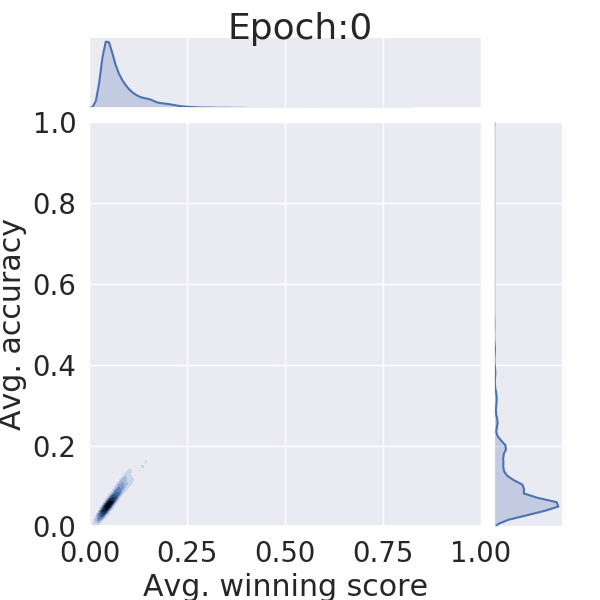
\includegraphics[width=\textwidth]{images/joint_plot/no_mixup/0.png}
         \caption{}
     \end{subfigure}
     \hfill
     \begin{subfigure}[b]{0.19\textwidth}
         \centering
         \noindent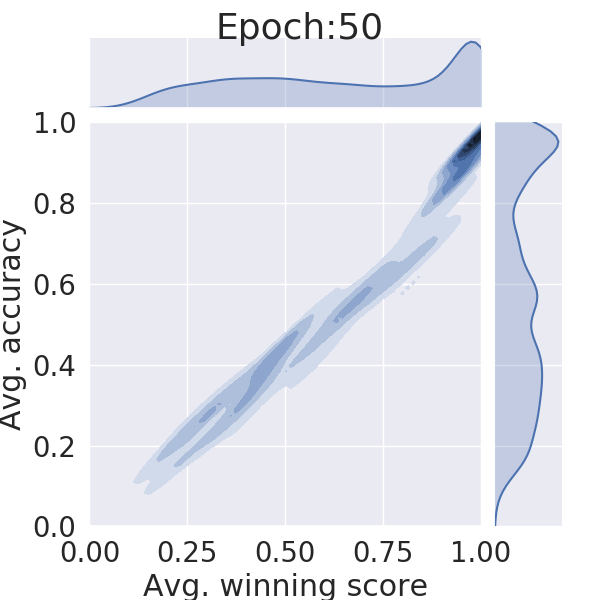
\includegraphics[width=\textwidth]{images/joint_plot/no_mixup/50.png}
         \caption{}
     \end{subfigure}
     \hfill
     \begin{subfigure}[b]{0.19\textwidth}
         \centering
         \noindent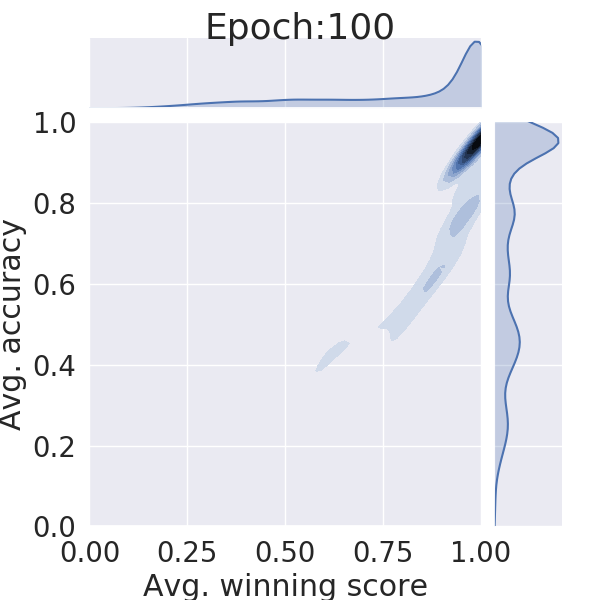
\includegraphics[width=\textwidth]{images/joint_plot/no_mixup/100.png}
         \caption{}
     \end{subfigure}
          \centering
     \begin{subfigure}[b]{0.19\textwidth}
         \centering
         \noindent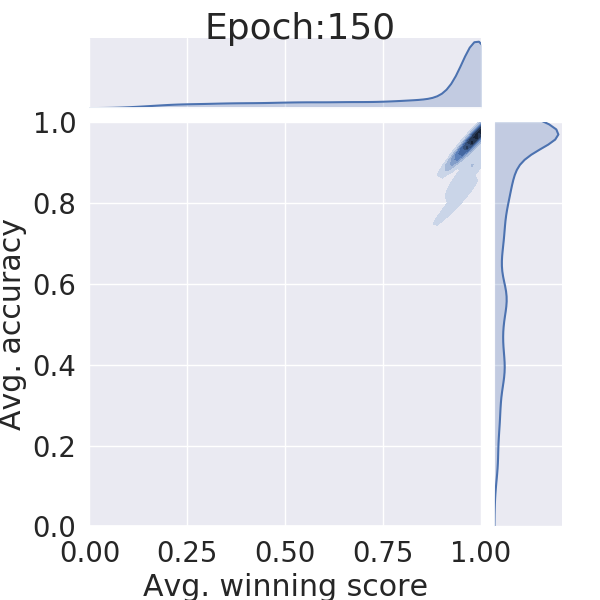
\includegraphics[width=\textwidth]{images/joint_plot/no_mixup/150.png}
         \caption{}
     \end{subfigure}
     \hfill
     \begin{subfigure}[b]{0.19\textwidth}
         \centering
         \noindent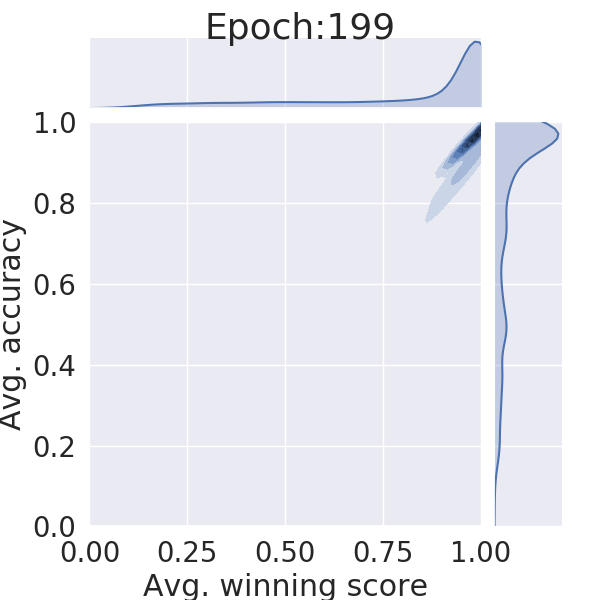
\includegraphics[width=\textwidth]{images/joint_plot/no_mixup/199.png}
         \caption{}
     \end{subfigure}
         \centering
     \begin{subfigure}[b]{0.19\textwidth}
         \centering
         \noindent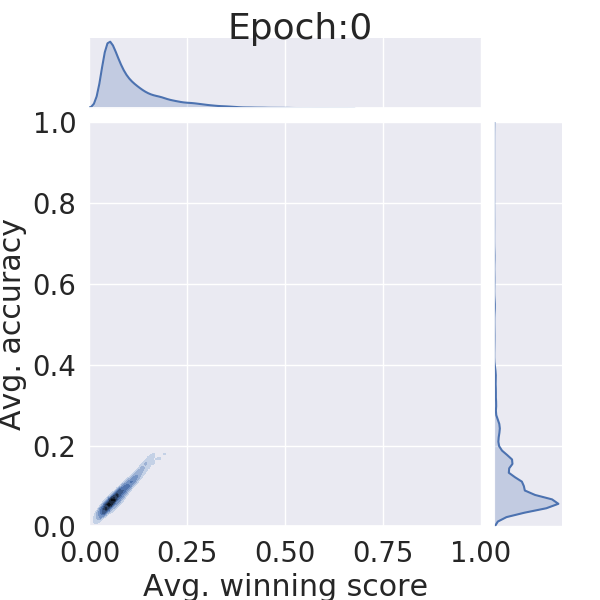
\includegraphics[width=\textwidth]{images/joint_plot/mixup/0.png}
         \caption{}
     \end{subfigure}
     \hfill
     \begin{subfigure}[b]{0.19\textwidth}
         \centering
         \noindent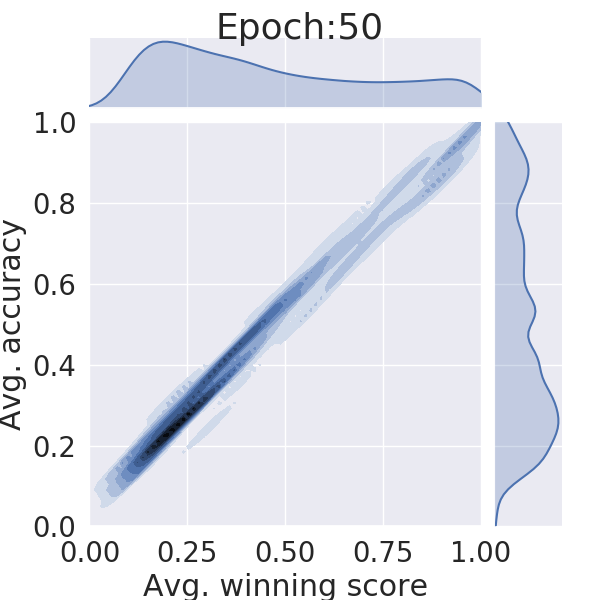
\includegraphics[width=\textwidth]{images/joint_plot/mixup/50.png}
         \caption{}
     \end{subfigure}
     \hfill
     \begin{subfigure}[b]{0.19\textwidth}
         \centering
         \noindent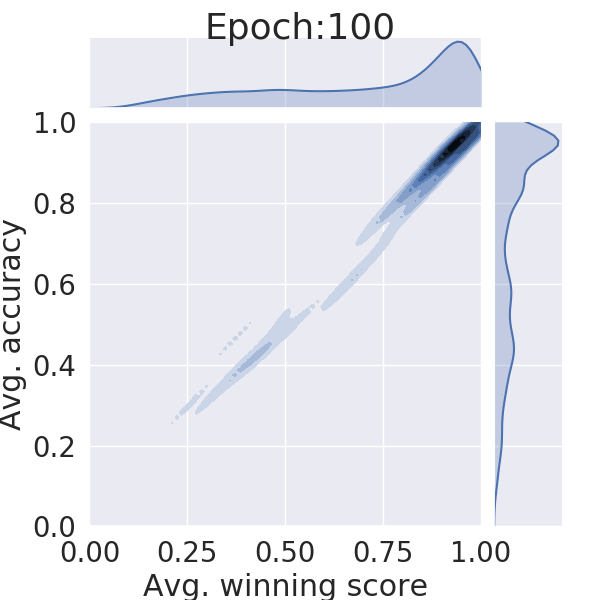
\includegraphics[width=\textwidth]{images/joint_plot/mixup/100.png}
         \caption{}
     \end{subfigure}
          \centering
     \begin{subfigure}[b]{0.19\textwidth}
         \centering
         \noindent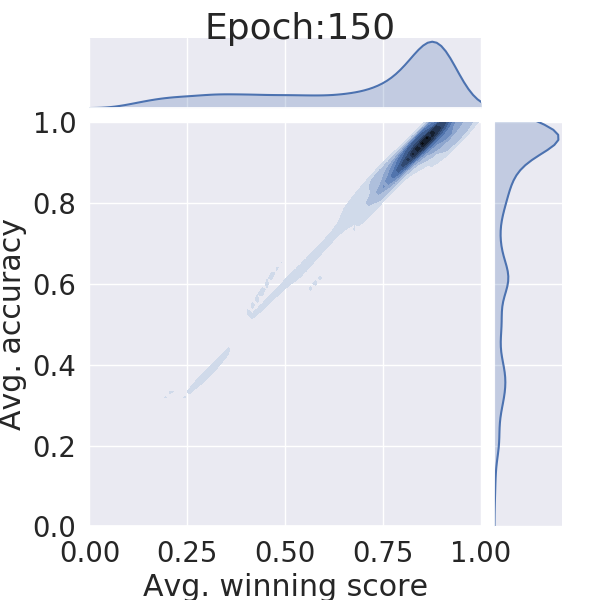
\includegraphics[width=\textwidth]{images/joint_plot/mixup/150.png}
         \caption{}
     \end{subfigure}
     \hfill
     \begin{subfigure}[b]{0.19\textwidth}
         \centering
         \noindent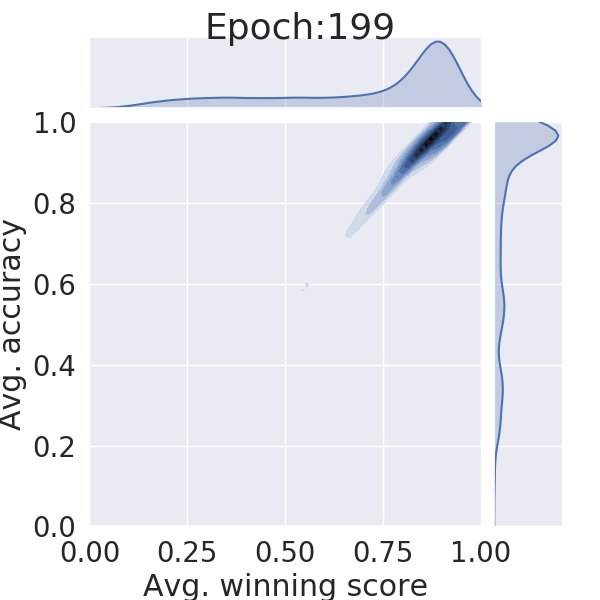
\includegraphics[width=\textwidth]{images/joint_plot/mixup/199.png}
         \caption{}
     \end{subfigure}
        \caption{Joint density plot for average accuracy vs average confidence computed for different epochs on CIFAR-100 test dataset using Resnet-34 neural network. \textbf{Top Row (a--e):} Trained without Mixup, the network grows overconfident as the training proceeds, as represented by the sharp peak for the confidence. \textbf{Bottom Row (f--j):} Mixup allows the network to be better calibrated in the corresponding epochs.}
        \label{fig:hypothesis}
\end{figure}

\subsection{Risk Minimisation and Mixup}
Given an input $\mathcal{X}$ and an output $\mathcal{Y}$ we are interested in finding $f \in \mathcal{F}$ which describes the mapping from input to the target output. The loss function $\ell$ penalises the differences between $f(x)$ and $y$ for samples $(x, y) \sim P(\mathcal{X}, \mathcal{Y})$. We aim to minimise the expected risk $\mathcal{R}$:
\begin{equation}
\mathcal{R}(\ell) = \int \ell(f(x), y)\; \mathrm{d}P(x, y).
\label{eq:rm}
\end{equation}
In most scenarios the joint probability distribution $P(x,y)$ is unavailable, and, subsequently, the task is altered to minimise the risk over the training data $\{(x_i,y_i)_{i=1}^{n}\}$. Therefore, $P$
%$\mathcal{P}$ 
is replaced by the empirical distribution $\hat{P}$, and this approach is referred to as Empirical Risk Minimisation (ERM) \cite{erm}. As a result of this substitution, equation \eqref{eq:rm} can be modified to find an approximate mapping $\hat{f} \in \mathcal{F}$ for $f$, as
\begin{equation}
\hat{\mathcal{R}}(\ell) = \int \ell(\hat{f}(x), y)\; \mathrm{d}\hat{P}(x, y),
\label{eq:erm}
\end{equation}
where
\begin{equation}
\hat{P}(x, y) = \frac{1}{n} \sum_{i=1}^{n} \delta(x=x_i, y=y_i),
\end{equation}
and $\delta(x=x_i, \;y=y_i)$ is a Dirac delta distribution centered at $x_i, y_i$. 

The vicinal probability distribution ${P}_v$ is the probability of finding a virtual feature-target pair
$ (\Tilde{x},\; \Tilde{y})$ in the vicinity of the original pair $(x_i,\; y_i)$. Since the support of $\hat{P}(x,y)$ is a one-point set, it fails to approximate $P(x,y)$ if $P$ is a continuous distribution \cite{vrm_0, vrm_1}. Vicinal Risk Minimisation (VRM) \cite{vrm_0} assumes that the input distribution is smooth in the vicinity of $x_i$, and replaces $\hat{P}$ by the vicinal probability distribution ${P}_v$, where
\begin{equation}
    \mathcal{P}_v = \frac{1}{n} \sum_{i=1}^{n} v(\Tilde{x}, \Tilde{y}\: |\: x_i,\; y_i).
\end{equation}
Mixup \cite{mixup_2018} is based on the principle of VRM, and generates the vicinal input and the corresponding target from a convex combination of a pair of original inputs and targets. Formally, the vicinal input and output can be represented as
\begin{align}
    &\Tilde{x}_i = \lambda x_i + (1-\lambda)x_j \\
    &\Tilde{y}_i = \lambda y_i + (1-\lambda)y_j,
\end{align}
where $x_i$ and $x_j$ are randomly selected input samples, $y_i$ and $y_j$ are their corresponding target values, and $\lambda \in [0, 1] $ is drawn from a symmetric $Beta\: distribution \:\mathcal{B}(\alpha, \alpha)$. The expected risk $\hat{R}_v$ for Mixup can thus be defined as
\begin{equation}
\hat{\mathcal{R}_v}(\ell) = \frac{1}{n}\sum_{i=1}^{n} \ell(\hat{f}(\Tilde{x}_i), \Tilde{y}_i).
\label{eq:vrm}
\end{equation}

\subsection{Proposed Method}
Mixup serves as simple yet effective data-augmentation procedure to enhance the performance of deep neural networks. The working of Mixup has been proved empirically via extensive experiments to suggest that its contribution in boosting the performance is significant. However, moving away from analysing the boost in performance or explaining why Mixup works, the authors explore the impact of Mixup on the calibration of deep neural networks. The paper performs considerable experiments across a number of datasets to measure the degree of miscalibration with Mixup and make a comparison with clearly defined baselines.

As part of the replication track of NeurIPS Reproducibility challenge 2019, we aim at reproducing the reported results of their hypothesis, i.e.\ training with Mixup leads to better calibrated neural networks. For the baseline, though not required by the track, we use training \textbf{without Mixup}. The report is structured as follows: Section \ref{sec:metrics} contains the description of the metrics used by the authors, in Section \ref{sec:implementation} we provide a detailed information of the implementations which we gathered from the authors' submission as well as email correspondences. We also state clearly where we make certain reasonable assumptions in implementation. Section \ref{sec:experiments} contains the results on various datasets. In the end, we provide our concluding remarks in Section \ref{sec:conclusion}.


\section{Calibration Metrics}
\label{sec:metrics}
To measure the calibration of a network, we follow the approach as described in \cite{calibration}. 
We initially define the number of confidence intervals $M$ each of size $1/M$. The confidence interval $I_m$ corresponds to the confidence range $\left((m-1)/M,\; m/M\right]$. Let $B_m$ be the set of samples for which the predicted confidence falls in $I_m$. The accuracy and confidence for $B_m$ are defined, respectively, as
\[ acc(B_m) = \frac{1}{|B_m|} \sum_{i \in B_m}\bm{1}(\hat{y}_i = y_i) \]
\[ conf(B_m) = \frac{1}{|B_m|} \sum_{i \in B_m}\hat{p}_i, \]
where $\hat{y}_i, y_i, \text{and}\; \hat{p}_i $ correspond to predicted label, true label, and the confidence (or winning score), respectively. Unless stated explicitly, confidence and accuracy will refer to a bin's confidence and accuracy.

The \textbf{Expected Calibration Error} (\textbf{ECE}) measures the amount of miscalibration in a network by computing the difference between the confidence and accuracy over the $M$ intervals. Formally, ECE is defined as
\[ ECE = \sum_{m=1}^{M} \frac{|B_m|}{n} \: \Big| conf(B_m) - acc(B_m)\Big|. \]

The \textbf{Overconfidence Error} (\textbf{OE}) is a weighted measure, which penalises overconfident predictions, and is defined as
\[ OE = \sum_{m=1}^{M} \frac{|B_m|}{n} \: \left[ conf(B_m) *max\left(conf(B_m)-acc(B_m),\: 0\right) \right]. \]


\section{Implementation Details}
\label{sec:implementation}
We have followed, wherever applicable, the implementation details of authors submission. Though, some of the fine grain details on training a network and generating the reported results were lacking, for this we have made reasonable assumptions and listed below a full table of implementation details, which we followed. The details are provided in Table \ref{tab:details}.

% \begin{tabular}{cc|c|c|l}
% \cline{3-4}
% & & \multicolumn{2}{ c| }{Networks(Resnet-18, Resnet-34, VGG-16)} \\ \cline{3-4}
% & & Value & Description  \\ \cline{1-4}
% \multicolumn{1}{ |c  }{\multirow{10}{*}{Attributes} } &
% \multicolumn{1}{ |c| }{Framework} & PyTorch & -- &     \\ \cline{2-4}
% \multicolumn{1}{ |c  }{}                        &
% \multicolumn{1}{ |c| }{Networks} & Resnet-18, Resnet-34, and VGG-16  &  --   \\ \cline{2-4}
% \multicolumn{1}{ |c  }{}                        &
% \multicolumn{1}{ |c| }{Datasets} & Fashion-MNIST, STL-10, Cifar-100, and MNIST &  --   \\ \cline{2-4}
% \multicolumn{1}{ |c  }{}                        &
% \multicolumn{1}{ |c| }{Batch normalisation} & Enabled & -- &     \\ \cline{2-4}
% \multicolumn{1}{ |c  }{}                        &
% \multicolumn{1}{ |c| }{Weight initialisation} & Kaiming & -- &     \\ \cline{2-4}
% \multicolumn{1}{ |c  }{}                        &
% \multicolumn{1}{ |c| }{Batch size} & 128 &  --   \\ \cline{2-4}
% \multicolumn{1}{ |c  }{}                        &
% \multicolumn{1}{ |c| }{Epochs} & 200 &  --   \\ \cline{2-4}
% \multicolumn{1}{ |c  }{}                        &
% \multicolumn{1}{ |c| }{Initial learning rate} & 0.1 & Halved at 60, 120, 160 epochs  \\ \cline{2-4}
% \multicolumn{1}{ |c  }{}                        &
% \multicolumn{1}{ |c| }{Optimiser} & SGD &  --   \\ \cline{2-4}
% \multicolumn{1}{ |c  }{}                        &
% \multicolumn{1}{ |c| }{Momentum} & 0.9 &    Nesterov momentum \\ \cline{2-4}
% \multicolumn{1}{ |c  }{}                        &
% \multicolumn{1}{ |c| }{Weight decay} & 0.0005 &    -- \\ \cline{2-4}
% \multicolumn{1}{ |c  }{}                        &
% \multicolumn{1}{ |c| }{Number of interval bins $M$} & 100 & --   \\ \cline{2-4}
% \multicolumn{1}{ |c  }{}                        &
% \multicolumn{1}{ |c| }{Data pre-processing} & Enabled & Random crops(padding=$4$), rotation $\SI{\pm 15}{}^\circ$, horizontal flips\\ \cline{1-4}
% \end{tabular}
%\begin{center}
\begin{table}[t]
\caption{Fine-grain details for replicating the experiments}\label{tab:details}
\begin{tabularx}{\textwidth}{XXX}
\toprule
Property & Values & Remark\\
\toprule
\rule{0pt}{1\normalbaselineskip}Framework & Pytorch & Version 1.3.1\\
\hline
\rule{0pt}{1\normalbaselineskip}Neural Networks & Resnet-18, Resnet-34, and VGG-16& --\\
\hline
\rule{0pt}{1\normalbaselineskip}Datasets & CIFAR-100, Fashion-MNIST, MNIST, and STL-10 & More details in their corresponding results sections\\
\hline
\rule{0pt}{1\normalbaselineskip}Batch Normalisation & Enabled & --\\
\hline
\rule{0pt}{1\normalbaselineskip}Weight Initialisation & Kaiming & Assumed as the detail was not provided in the report \\
\hline
\rule{0pt}{1\normalbaselineskip}Batch Size & $128$ & --\\
\hline
\rule{0pt}{1\normalbaselineskip}Epochs & $200$ & --\\
\hline
\rule{0pt}{1\normalbaselineskip}Initial Learning Rate & 0.1 & Reduced by a factor of $0.5$ at $60, 120, 160$ epoch\\
\hline
\rule{0pt}{1\normalbaselineskip}Optimiser & SGD & --\\
\hline
\rule{0pt}{1\normalbaselineskip}Momentum & $0.9$ & Nesterov momentum\\
\hline
\rule{0pt}{1\normalbaselineskip}Weight Decay & $5\text{x}10^{-4}$ & --\\
\hline
\rule{0pt}{1\normalbaselineskip}Number of Interval Bins & 100 & Communicated via email by the authors\\
\hline
\rule{0pt}{1\normalbaselineskip}Data Pre-processing & Enabled & Random cropping(padding=$4$), rotation $\SI{\pm 15}{}^\circ$, horizontal flipping, standardisation \\
\bottomrule
\end{tabularx}
\end{table}
%\end{center}


\section{Replication Experiments}
\label{sec:experiments}
% \subsection{Degree of Calibration in Training}
% This experiment is to highlight the stark difference between networks trained with and without Mixup. The joint density plot in \ref{fig:joint_plot} depicts the calibration over the training phase. For this, accuracy and confidence are utilised as defined in equations \ref{eq:acc, eq:conf} for $M=100$ bins. Figure \ref{fig:joint_plot} a-e represent the training for a network \textbf{without} Mixup and as we can notice the predictions tend to become overconfident at the last epoch. In figure \ref{fig:joint_plot} f-i, representing the training with Mixup(alpha=0.3), the network appears to be better calibrated in the corresponding epochs. \newline
% Trends of the joint density plots are inline with the results reported by the authors. 
We conduct $4$ trials per experiment, and report the mean and standard deviation over the trials. We report results for more than few values of $\alpha$ as opposed to the paper. The authors report the best working value of $\alpha \in \lbrack 0.2, 0.4 \rbrack $ hence, we use $\alpha=0.3$ when selecting an individual value for $\alpha$. Accuracy, ECE, and OE are computed for $\alpha \in [0, 1]$. Important thing to note is $\alpha = 0$ corresponds to \textbf{no Mixup}, which is one of the author's baseline, and $\alpha=1$ is simple averaging of two input images. %The addition of $\pm$ standard deviation also provides additional insights as to the range of values for accuracy, ECE and OE one can expect which are missing from the paper.
Including $\pm$ standard deviation also provides additional insights to the range of values for accuracy, ECE and OE which are, instead, missing in the paper.
We also show scatter plots for $\alpha=\{0, 0.3, 1.0\}$ to compare average bin accuracy against average bin confidence. To provide additional details of the frequency of samples in the bin, we scale the point size on the plot to correspond to the size of the bin $|B_m|$.


\subsection{CIFAR-100}
CIFAR-100 consists of $100$ classes with input images of dimensions $32\text{x}32\text{x}3$. We use the standard split of the dataset consisting of $50,000$ and $10,000$ as training and test images, respectively. We train the Resnet-34 model following the details provided in the Section \ref{sec:implementation}. 

The results can be viewed in Figure \ref{fig:cifar100}. Though we were not able to obtain the accuracy value $~80\%$, we were able to replicate the trend that the accuracy is higher when the network is trained with Mixup. For ECE and OE there are significant fluctuations in the values. The results reported by the authors lie within one standard deviation due to large value of standard deviation. However, ECE decreases till $\alpha=0.3$ and then increases, which is also reported in paper. Figure \ref{fig:cifar100} (d--f) represents the shift from the network being overconfident ($\alpha=0$) to under confident ($\alpha=1$). The network is better calibrated, if the points in the scatter plot lie close to the line $y=x$, and it is observed with $\alpha=0.3$ in Figure \ref{fig:cifar100} (e).
\begin{figure}[h]
     \centering
     \begin{subfigure}[b]{0.31\textwidth}
         \centering
         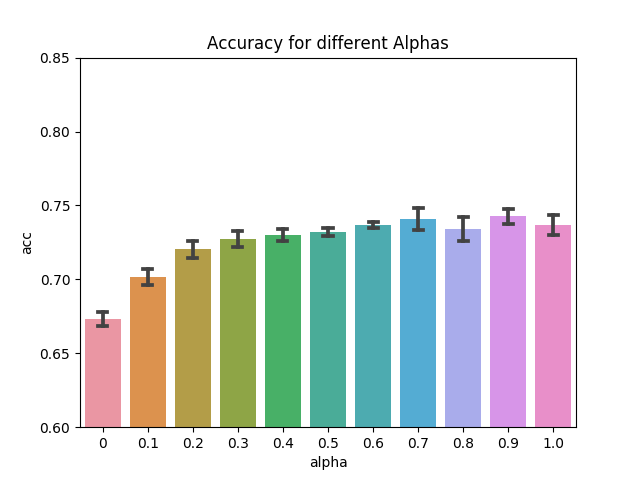
\includegraphics[width=\textwidth]{images/cifar/accuracyValpha.png}
         \caption{Accuracy for different $\alpha$}
     \end{subfigure}
     \begin{subfigure}[b]{0.31\textwidth}
         \centering
         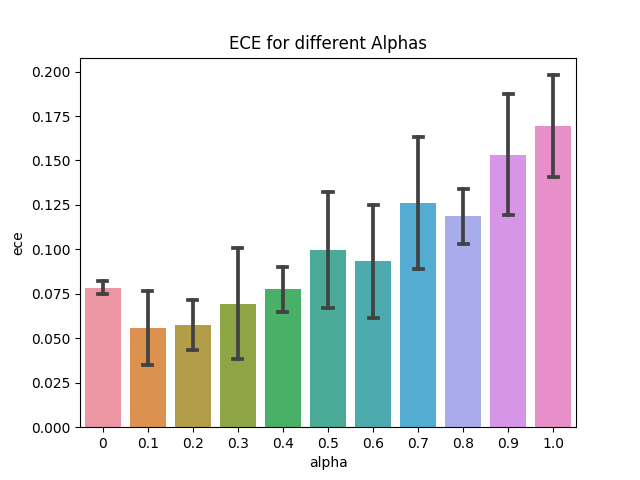
\includegraphics[width=\textwidth]{images/cifar/eceValpha.png}
         \caption{Expected Calibration Error}
     \end{subfigure}
     \begin{subfigure}[b]{0.31\textwidth}
         \centering
         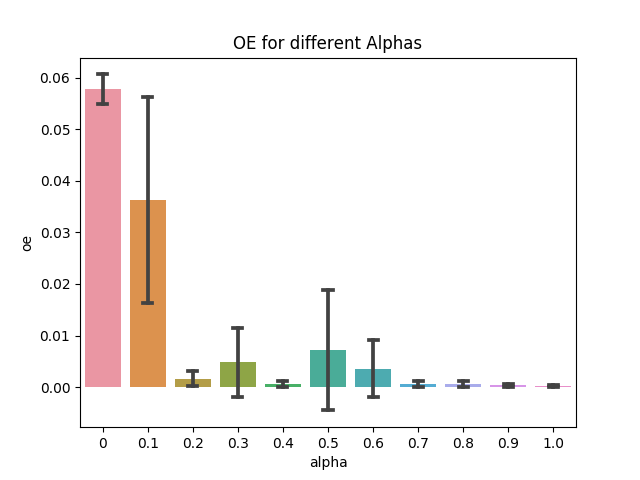
\includegraphics[width=\textwidth]{images/cifar/oeValpha.png}
         \caption{Overconfidence error}
     \end{subfigure}
     \begin{subfigure}[b]{0.31\textwidth}
         \centering
         \noindent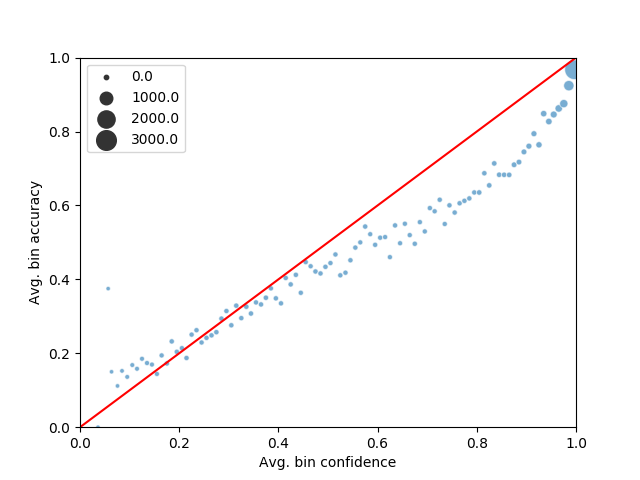
\includegraphics[width=\textwidth]{images/cifar/scatterplot_0.png}
         \caption{No Mixup ($\alpha=0$)}
     \end{subfigure}
     \begin{subfigure}[b]{0.31\textwidth}
         \centering
         \noindent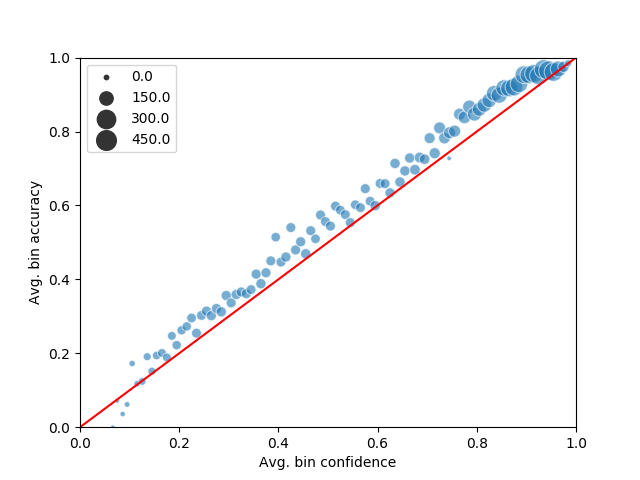
\includegraphics[width=\textwidth]{images/cifar/scatterplot_0_3.png}
         \caption{$\alpha=0.3$}
     \end{subfigure}
     \begin{subfigure}[b]{0.31\textwidth}
         \centering
         \noindent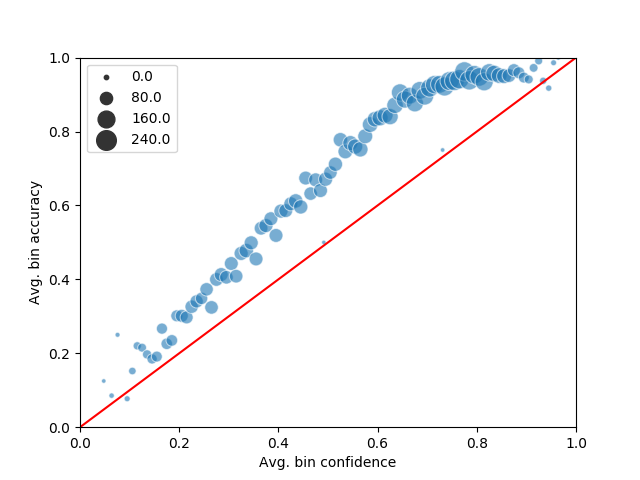
\includegraphics[width=\textwidth]{images/cifar/scatterplot_1.png}
         \caption{Simple average ($\alpha=1$)}
     \end{subfigure}
        \caption{Replication of the results corresponding to CIFAR-100 dataset.}
        \label{fig:cifar100}
\end{figure}

\subsection{STL-10}
The dataset consists of labelled as well as unlabelled examples. For the purpose of this experiment, we utilise the labelled split of train and test. The dataset consists of $10$ classes with input images of dimensions $96\text{x}96\text{x}3$. We train the VGG-16 model following the details provided in the Section \ref{sec:implementation}.

The accuracy matches with the values reported by authors as observed in Figure \ref{fig:stl_10}. The trend of improved accuracy due to Mixup is also observed. For ECE, and OE the values for no Mixup were off, but the expected trend of improved calibration was observed. Again, $\alpha \in \lbrack 0.2, 0.4 \rbrack $ can be seen as the best value w.r.t ECE. Figure \ref{fig:stl_10} (d--f) represents the shift from the network being overconfident ($\alpha=0$) to under confident ($\alpha=1$). 

\begin{figure}[h]
     \centering
     \begin{subfigure}[b]{0.31\textwidth}
         \centering
         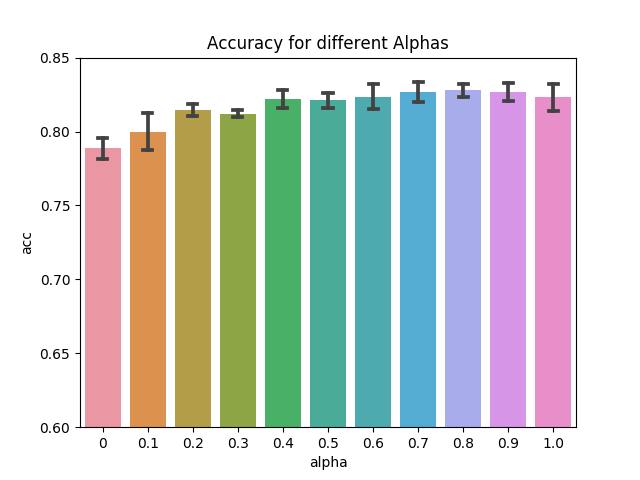
\includegraphics[width=\textwidth]{images/stl10/accuracyValpha.png}
         \caption{Accuracy for different $\alpha$}
     \end{subfigure}
     \begin{subfigure}[b]{0.31\textwidth}
         \centering
         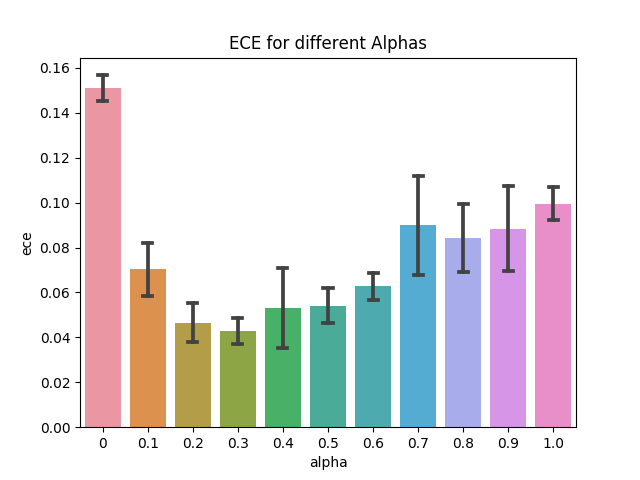
\includegraphics[width=\textwidth]{images/stl10/eceValpha.png}
         \caption{Expected Calibration Error}
     \end{subfigure}
     \begin{subfigure}[b]{0.31\textwidth}
         \centering
         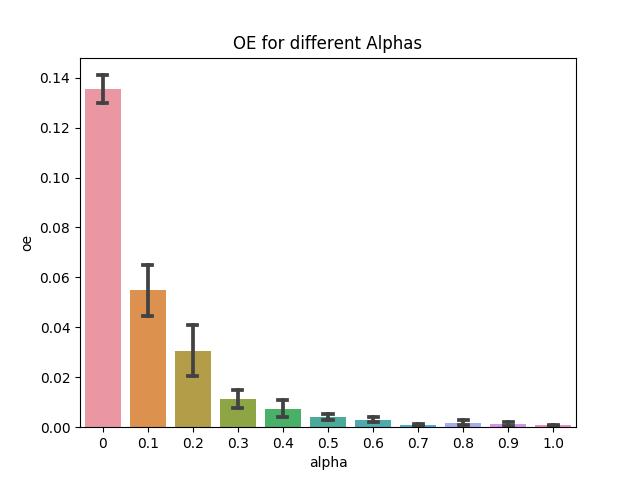
\includegraphics[width=\textwidth]{images/stl10/oeValpha.png}
         \caption{Overconfidence Error}
     \end{subfigure}
     \begin{subfigure}[b]{0.31\textwidth}
         \centering
         \noindent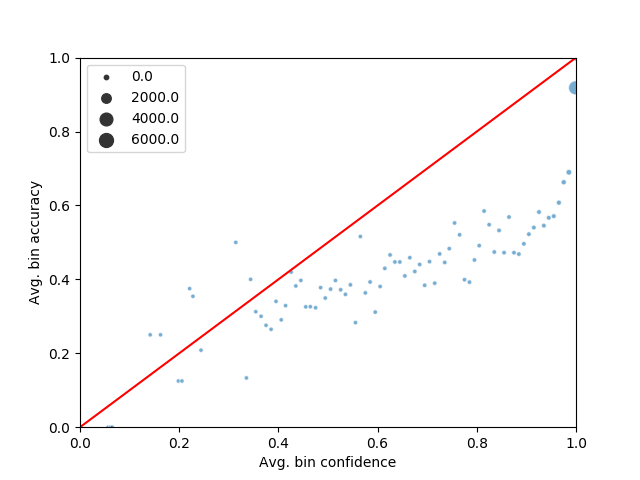
\includegraphics[width=\textwidth]{images/stl10/scatterplot_0.png}
         \caption{No Mixup ($\alpha=0$)}
     \end{subfigure}
     \begin{subfigure}[b]{0.31\textwidth}
         \centering
         \noindent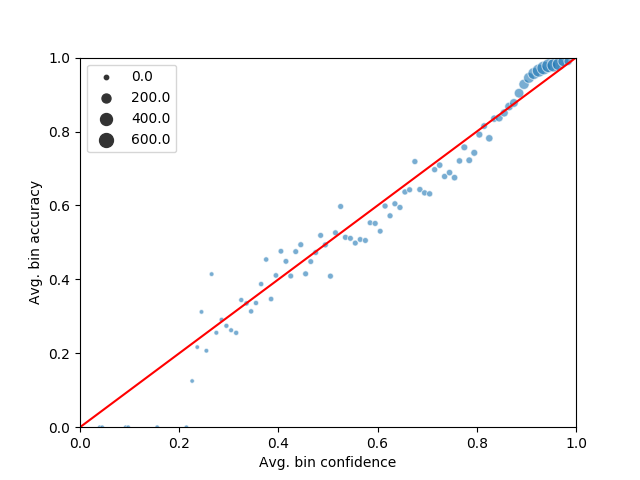
\includegraphics[width=\textwidth]{images/stl10/scatterplot_0-3.png}
         \caption{$\alpha=0.3$}
     \end{subfigure}
     \begin{subfigure}[b]{0.31\textwidth}
         \centering
         \noindent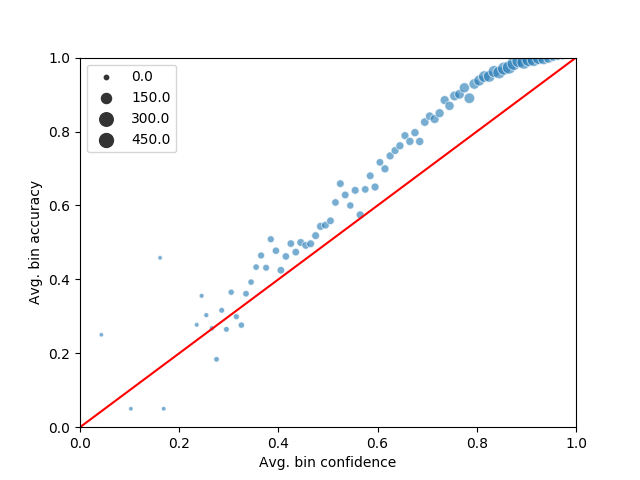
\includegraphics[width=\textwidth]{images/stl10/scatterplot_1.png}
         \caption{Simple average ($\alpha=1$)}
     \end{subfigure}
        \caption{Replication of the results for STL-10 dataset.}
        \label{fig:stl_10}
\end{figure}

\subsection{Fashion-MNIST}
The dataset consists of a training set of $60,000$ examples and a test set of $10,000$ examples. Each example is a $28\text{x}28\text{x}1$ gray-scale image, associated with a label from $10$ classes. We use the standard splits for training and testing. 

The effect of Mixup on accuracy are not quite evident, since the network learns to classify effectively even without Mixup, Figure \ref{fig:fmnist}. ECE value is lower for majority of $\alpha$ indicating better calibration. The scatter-plot is not a good indicator to analyse the calibration in this case as majority of the samples are easily classified by the neural network with high accuracy. Only OE behaves a expected suggesting that Mixup helps in calibrating the neural network to avoid over confident predictions.    
\begin{figure}[h]
     \centering
     \begin{subfigure}[b]{0.31\textwidth}
         \centering
         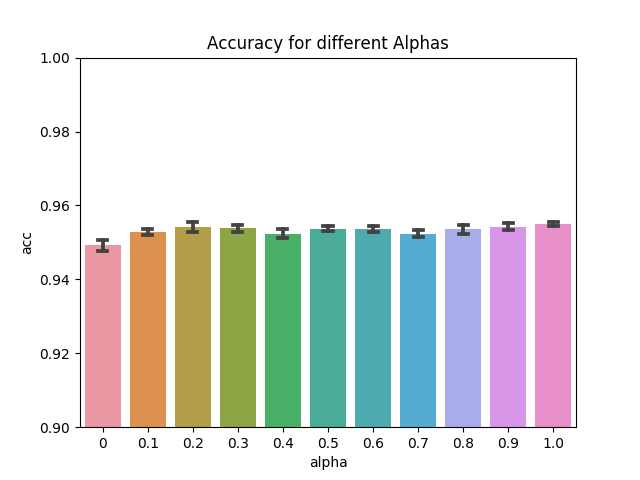
\includegraphics[width=\textwidth]{images/fmnist/accuracyValpha.png}
         \caption{Accuracy for different $\alpha$}
     \end{subfigure}
     \begin{subfigure}[b]{0.31\textwidth}
         \centering
         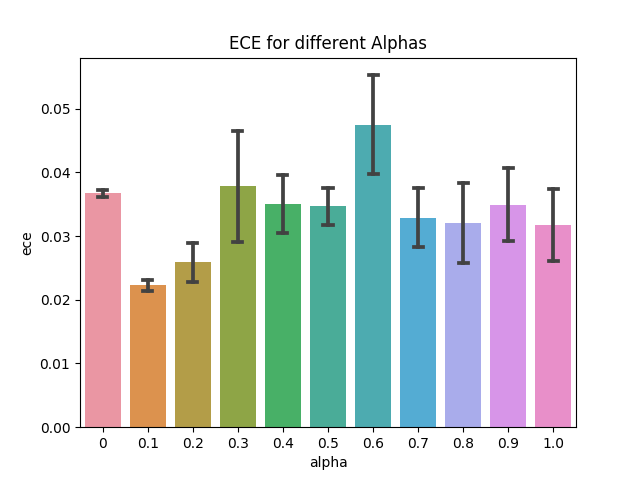
\includegraphics[width=\textwidth]{images/fmnist/eceValpha.png}
         \caption{Expected Calibration Error}
     \end{subfigure}
     \begin{subfigure}[b]{0.31\textwidth}
         \centering
         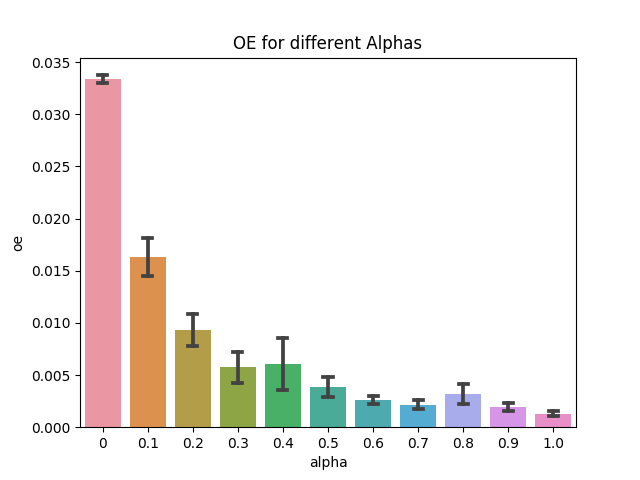
\includegraphics[width=\textwidth]{images/fmnist/oeValpha.png}
         \caption{Overconfidence error}
     \end{subfigure}
     \begin{subfigure}[b]{0.31\textwidth}
         \centering
         \noindent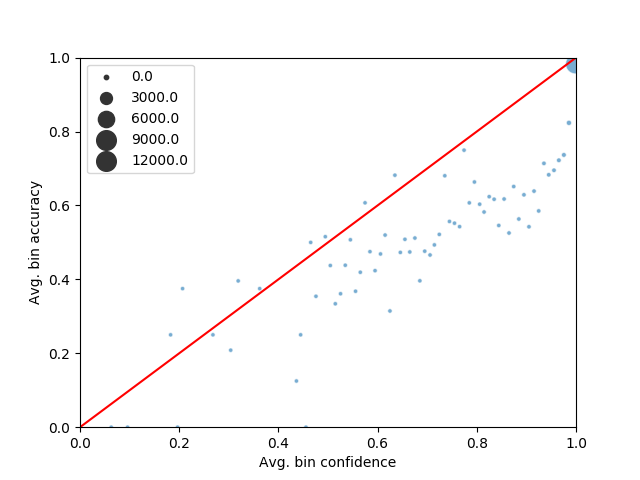
\includegraphics[width=\textwidth]{images/fmnist/scatterplot_0.png}
         \caption{No Mixup ($\alpha=1$)}
     \end{subfigure}
     \begin{subfigure}[b]{0.31\textwidth}
         \centering
         \noindent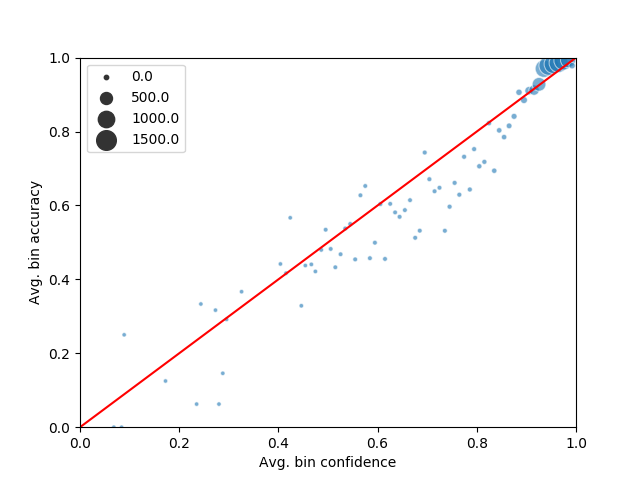
\includegraphics[width=\textwidth]{images/fmnist/scatterplot_0-3.png}
         \caption{$\alpha=0.3$}
     \end{subfigure}
     \begin{subfigure}[b]{0.31\textwidth}
         \centering
         \noindent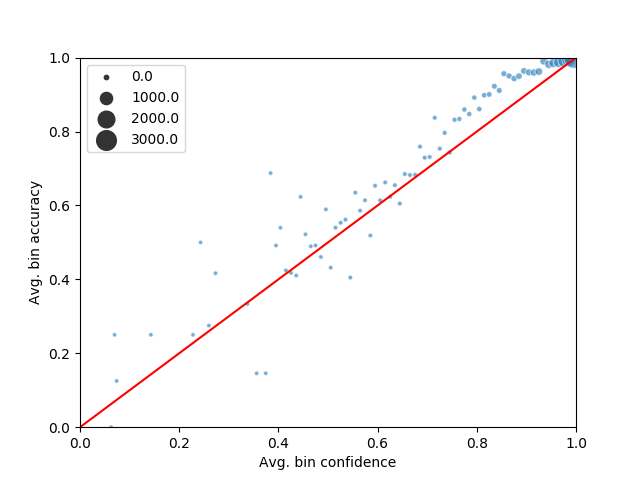
\includegraphics[width=\textwidth]{images/fmnist/scatterplot_1.png}
         \caption{Simple average ($\alpha=1$)}
     \end{subfigure}
        \caption{Replication of the results for Fashion-MNIST dataset.}
        \label{fig:fmnist}
\end{figure}

\subsection{Testing on Out-Of-Distribution dataset \& Random Noise}
\label{sec:ood}
In the original work, authors have trained a neural network on STL-10 (in-distribution data) and tested on the samples from ImageNet (out-of-distribution data) \cite{imagenet_cvpr09}, corresponding to new classes only. On the other hand, we aim to replicate the effectiveness of this experiment by training on Fashion-MNIST (in distribution data) and test on MNIST (out-of-distribution data). In principle, the findings of our experiment should go along with the reported results.

MNIST, similar to Fashion-MNIST, consists of $50,000$ training and $10,000$ test images of dimensions $28\text{x}28\text{x}3$. We train the Resnet-18 network on the train split of Fashion-MNIST and report the results on the test split of MNIST. For random noise images, we use Gaussian noise with mean and standard deviation of the Fashion-MNIST dataset to generate $1024$ test images. 

In Figure \ref{fig:out_dist}, the plots closely resemble to the outputs of the paper. For both the scenarios, we can observe that the network trained with Mixup is significantly less confident in predicting the test samples. For random noise, the predictions are somewhat separable as reported by the authors. 
\begin{figure}[h]
     \centering
     \begin{subfigure}[b]{0.45\textwidth}
         \centering
         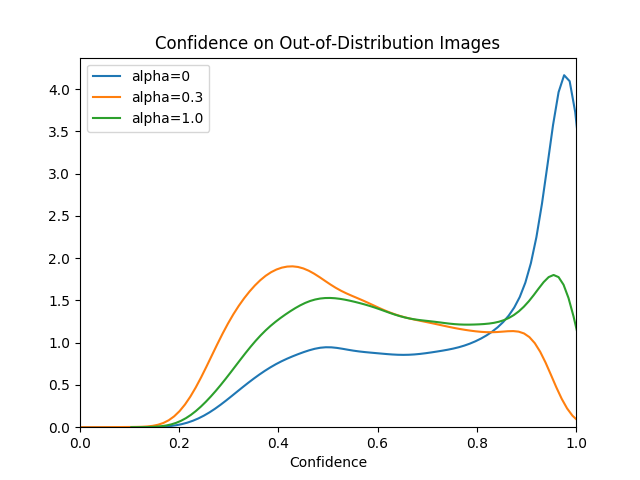
\includegraphics[width=\textwidth]{images/ood/distplot.png}
         \caption{Out-of-Distribution data}
     \end{subfigure}
     \begin{subfigure}[b]{0.45\textwidth}
         \centering
         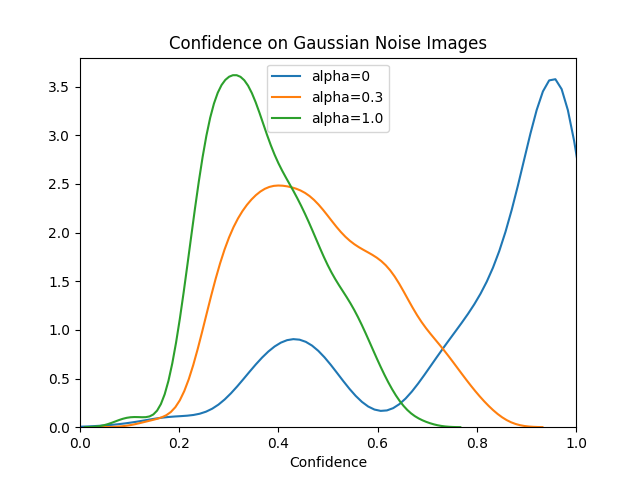
\includegraphics[width=\textwidth]{images/noise/distplot.png}
         \caption{Gaussian noise data}
     \end{subfigure}
        \caption{Distribution of confidence of various models when tested on out-of-distribution and Gaussian noise samples, after being trained on the Fashion-MNIST dataset}
        \label{fig:out_dist}
\end{figure}


\section{Conclusion}
\label{sec:conclusion}
In this report, we were able to confirm the main
% major 
results reported in \cite{onmixup} by replicating the majority of the experiments. Though the values were not exactly replicated for ECE and OE, the trend of improved calibration when the network is trained using Mixup was confirmed. We were able to obtain the authors finding regarding the value of $\alpha \in [0.2, 0.4]$, providing the best calibration in terms of ECE. Through the out-of-distribution and random noise experiments in Section \ref{sec:ood}, we were able to provide some evidence regarding the generalisability of the author's corresponding experiment, thereby strengthening their claim of improved calibration on unseen data. The decrease of OE with increase in $\alpha$ is also confirmed, which the authors attributed to underfitting of the model. An important finding from the replication of the experiments was the volatility of the error values, hence we urge future researchers to report mean and variance for the errors to allow for better comparisons. We also provide our source code \footnote{https://github.com/MacroMayhem/OnMixup} for generating the results and setting up the experiments.
